\chapter{El caso infinito}
\label{chap:inf}

% TODO: resumen del capítulo

\noindent
Sea $\vec{p} \in \R^n \setminus \braces{\vec{0}}$ un vector esencialmente entero y recordemos de la
definición \ref{theory:def:rational} que tiene un único múltiplo coprimo $\vec{q} \in \Z^n$. Es
decir, existe un único escalar $m \in \R$ que satisface tres cosas: $\vec{p} = m\vec{q}$, las
entradas $q_1, \ldots, q_n$ son coprimas, y la primera entrada no nula $q_i$ es positiva. Al igual
que en el capítulo anterior, supondremos que $m$ es positivo. Equivalentemente, supondremos que la
primera entrada no nula $p_i$ es positiva\footnote{ El autor hace recordar que esta es una cuestión
	puramente de comodidad y no hay pérdida de generalidad. Cuando $m$ es negativo, los resultados
se mantienen pero es necesario voltear las desigualdades y cambiar las funciones piso por las
funciones techo, lo cual añadiría un número innecesario de casos a analizar.}.

Retomemos el entero $\eta \in \Z$ del lema \ref{phase-1:lemma:eta} que parametriza la primera capa
entera que satisface el presupuesto \eqref{theory:constraint:budget}. A causa del teorema
\ref{theory:th:feasibility} sabemos que si $q_i \leq 0$ para alguna $i \in \braces{1, \ldots, n}$,
entonces la $\eta$-ésima capa entera contiene un número infinito de puntos factibles. A partir de
esto último, somos capaces de resolver el automáticamente el problema de decisión de determinar si
un escalar $u^* \in \R$ es el valor óptimo del programa (\ref{theory:formulation}).
\begin{corollary}
	\label{cor:inf:obj}
	Supongamos que $q_i \leq 0$ para algún $i \in \braces{1, \ldots, n}$. Entonces el valor óptimo
	del programa lineal entero (\ref{theory:formulation}) es $m\eta$. Además, si $m$ es positivo,
	tenemos que $\eta$ es el múltiplo de $m$ más grande que satisface $m\eta \leq u$, donde $u$ es
	el lado derecho de la restricción presupuestaria \eqref{theory:constraint:budget}.
\end{corollary}
\begin{proof}
	Por el teorema \ref{theory:th:feasibility} sabemos que existen una infinidad de soluciones en la
	$\eta$-ésima capa entera, así que sea $\vec{x}^*$ una de ellas. Entonces $\vec{q}^T\vec{x}^* =
	\eta$, pero $\vec{p} = m\vec{q}$ por la definición \ref{theory:def:rational}, por lo que
	obtenemos $\vec{p}^T\vec{x}^* = m\vec{q}^T\vec{x}^* = m\eta$.

	Ahora bien, si $m$ es positivo, por el lema \ref{phase-1:lemma:eta} tenemos que
	$\eta = \lfloor u/m \rfloor$
	. Supongamos que $\xi \in \Z$ satisface $m\xi \leq u$ y también $\lfloor
	u/m \rfloor < \xi$. Luego,
	\begin{equation*}
		m\left\lfloor \frac{u}{m} \right\rfloor < m\xi \leq u
		\implies \left\lfloor \frac{u}{m} \right\rfloor < \xi \leq \frac{u}{m},
	\end{equation*}
	pero esto contradice las propiedades de la función piso.
\end{proof}

\begin{observation}
	Para ilustrar la conveniencia de restringir $m$ a que sea positivo, consideremos el caso cuando
	$m < 0$. De una manera similar a la del lema \ref{phase-1:lemma:eta}, podemos demostrar que
	$\eta \coloneq \lceil u/m \rceil$ parametriza también la primera capa entera que satisface el
	presupuesto, pues ahora tenemos de la restricción \eqref{theory:constraint:budget} que
	$\vec{p}^T\vec{x} \leq u$ si y solo si $\vec{q}^T\vec{x} \geq u/m$. Se sigue cumpliendo que el
	valor óptimo del problema \eqref{theory:formulation} es $m\eta$. Sin embargo, $\eta$ ahora es el
	múltiplo más chico de $m$ que satisface $m\eta \geq u$.
\end{observation}

Una vez resuelto el problema de decisión, podemos preguntarnos concretamente cómo obtener el punto
óptimo. Por el teorema \ref{theory:th:feasibility} sabemos que debemos resolver la ecuación lineal
diofantina $\vec{q}^T\vec{x} = \eta$. Del teorema \ref{th:lattice} sabemos que si $q_n \neq 0$,
entonces existen $k \in \Z$ y $\vec{t} \in \Z^{n-1}$ tales que
\begin{equation*}
	\vec{x} = k\vec{\nu} + M\vec{t},
\end{equation*}
donde $\vec{\nu}$ y $M$ están definidas por \eqref{eq:vec-omega} y \eqref{eq:mat-T},
respectivamente. De los lemas \ref{lemma:iso1} y \ref{lemma:iso2} sabemos que
\begin{equation*}
	\vec{q}^T\left(\eta\vec{\nu} + M\vec{t}\right) = \eta\vec{q}^T\vec{\nu} + \vec{q}^TM\vec{t} = \eta
\end{equation*}
para todo $\vec{t} \in \Z^{n-1}$. Así pues, debe ser el caso que $k = \eta$ y debemos encontrar
condiciones suficientes en $\vec{t}$ para asegurar la no-negatividad de $\vec{x}$. En primer lugar,
sabemos que para todo $i \in \braces{1, \ldots, n - 2}$, la entrada $t_i$ debe satisfacer
\eqref{eq:param-lb}. En segundo lugar, recuperamos de \eqref{eq:last-solution} que las últimas dos
soluciones de la ecuación $\vec{q}^T\vec{x} = \eta$ están dadas por
\begin{equation*}
	\begin{cases}
		x_{n-1} = \omega_{n-1}x_{n-1}' + \frac{q_n}{\prod_{j=1}^{n-1}g_j}t_{n-1}, \\
		x_n = \omega_{n-1}x_n' - \frac{q_{n-1}}{\prod_{j=1}^{n-1}g_j}t_{n-1},
	\end{cases}
\end{equation*}
donde los enteros $g_i$ están definidos por \eqref{dummy:next-g} con $g_1 = 1$, $\omega_{n-1}$ está
definida a través de la relación de recurrencia \eqref{eq:omega-recurrence} con condición inicial
$\omega_1 = \eta$ (o bien a partir del lema \ref{eq:omega-formula} con $k = \eta$), y $x_{n-1}',
x_n'$ son coeficientes de Bézout que satisfacen \eqref{eq:last-equation-bez}.

En lo que se encuentra a continuación supondremos que ninguna entrada $q_i$ es nula. Esto no
constituye problema alguno debido a un razonamiento similar al de la demostración del teorema
\ref{theory:th:feasibility}. Definimos
\begin{equation*}
	I^\circ \coloneq \braces{i \colon q_i = 0},
\end{equation*}
y también definimos el vector $\tvec{q}$ cuyas entradas son las entradas no nulas de
$\vec{q}$. A partir de lo que sigue vamos a determinar un vector entero no nulo $\tvec{x}$
que satisfaga $\tvec{q}^T\tvec{x} = \eta$. Luego, encontramos que el vector $\vec{x}$
dado por
\begin{equation*}
	x_i \coloneq
	\begin{cases}
		\tilde{x}_i, & i \not \in I^\circ, \\
		0, & i \in I^\circ,
	\end{cases}
\end{equation*}
es entero, no negativo, y también satisface $\vec{q}^T\vec{x} = \eta$. Así pues, la suposición de
que $q_i \neq 0$ para todo $i \in \braces{1, \ldots, n}$ toma lugar sin pérdida de generalidad.

Para que se satisfagan las condiciones de no negatividad de $x_{n-1}$ y de $x_n$, encontramos que
$t_{n-1} \in \Z$ debe cumplir ciertas desigualdades según los signos de $q_{n-1}$ y de $q_n$.
Definamos, por conveniencia,
\begin{equation}
	\label{eq:lr-bounds}
	b_1 \coloneq -\frac{\omega_{n-1}x_{n-1}'}{q_n} \cdot \prod_{j=1}^{n-1}g_j, \quad
	b_2 \coloneq \frac{\omega_{n-1}x_{n}'}{q_{n-1}} \cdot \prod_{j=1}^{n-1}g_j.
\end{equation}
Entonces, para asegurar la no-negatividad de $x_{n - 1}$ y de $x_n$, debe ser el caso que
\begin{equation}
	\label{eq:feasible-param}
	t_{n-1} \in 
	\begin{cases}
		\big[ \lceil \max\lbrace b_1 ,  b_2 \rbrace \rceil, \infty \big), &  q_{n-1} < 0 < q_n, \\[0.5em]
		\big( -\infty, \lfloor \min\lbrace b_1, b_2\rbrace \rfloor \big], &  q_n < 0 < q_{n-1}, \\[0.5em]
		\big[ \lceil b_2 \rceil, \lfloor b_1 \rfloor \big], &  q_{n-1}, q_n < 0, \\[0.5em]
		\big[ \lceil b_1 \rceil, \lfloor b_2 \rfloor \big], &  0 < q_{n-1}, q_n.
	\end{cases}
\end{equation}

Podemos emplear la misma estrategia de permutar las entradas de $q_i$ de manera que colapsemos estos
cuatro casos distintos en uno solo. Como estamos en el caso infinito del teorema
\ref{theory:th:feasibility}, naturalmente supondremos que $q_i < 0$ para alguna $i \in \braces{1,
\ldots n}$. Así pues, podemos permutar esta $i$-ésima entrada de $\vec{q}$ con $q_{n-1}$, con lo que
obtenemos $q_{n-1} < 0$. Luego, como $\vec{q}$ es el múltiplo coprimo de $\vec{p}$ y ninguna entrada
de $\vec{q}$ es nula, se sigue de la definición \ref{theory:def:rational} que $q_1 > 0$. Así pues,
podemos permutar la primera y última entrada de $\vec{q}$, de donde se sigue que $q_n > 0$.
Juntándolo todo, obtenemos $q_{n-1} < 0 < q_n$. De esta manera, para asegurar la no negatividad de
$x_{n-1}$ y $x_n$, basta con que se satisfaga el primer caso:
\begin{equation}
	\label{eq:feasible-param:collapsed}
	t_{n-1} \geq \ceil{\max\lbrace b_1, b_2 \rbrace}.
\end{equation}

\begin{lemma}
	\label{lemma:t-existence}
	Sea $\vec{p} \in \R$ un vector cuyas entradas son todas distintas de cero, y sea $\vec{q} \in
	\Z^n$ su múltiplo coprimo. Entonces existe un vector $\vec{t} \in \Z^{n-1}$ que satisface ambos
	\eqref{eq:param-lb} y \eqref{eq:feasible-param}.
\end{lemma}
\begin{proof}
	Por la discusión anterior, podemos suponer sin pérdida de generalidad que $q_{n-1} < 0 < q_n$,
	así que basta mostrar la existencia de  $\vec{t} \in \Z^{n-1}$ que satisfaga \eqref{eq:param-lb} y
	\eqref{eq:feasible-param:collapsed}. Si definimos
	\begin{equation*}
		t_i \coloneq \begin{cases}
			\ceil{-\frac{\omega_ix_i'}{g_{i + 1}}}, & i < n - 1, \\[0.5em]
			\ceil{\max\lbrace b_1, b_2 \rbrace}, & i = n - 1,
		\end{cases}
	\end{equation*}
	entonces se verifica automáticamente que estas condiciones se satisfacen.
\end{proof}

% \begin{lemma}
% 	\label{lemma:t-existence}
% 	Sea $\vec{p} \in \R$ un vector cuyas entradas son todas distintas de cero, y sea $\vec{q} \in
% 	\Z^n$ su múltiplo coprimo. Entonces existe un vector $\vec{t} \in \Z^{n-1}$ que satisface ambos
% 	\eqref{eq:param-lb} y \eqref{eq:feasible-param}.
% \end{lemma}
% \begin{proof}
% 	Tenemos cuatro casos, pero observemos que los dos en donde $q_{n - 1}$ y $q_n$
% 	tienen signo distinto no son difíciles: si $q_{n - 1} <0 < q_n$, entonces el vector
% 	$\vec{t} \in \Z^{n-1}$ dado por
% 	\begin{equation*}
% 		t_i \coloneq \begin{cases}
% 			\left\lceil -\frac{\omega_ix_i'}{g_{i + 1}} \right\rceil, & i < n - 1, \\[0.5em]
% 			\lceil \max\lbrace b_1, b_2 \rbrace \rceil, & i = n - 1,
% 		\end{cases}
% 	\end{equation*}
% 	satisface ambos (\ref{eq:param-lb}) y (\ref{eq:feasible-param}). El caso $q_n < 0 <
% 	q_{n - 1}$ es completamente similar.
% 
% 	Consideremos el caso $q_{n - 1}, q_n < 0$. Como ninguna entrada de $\vec{p}$ es nula y el vector
% 	$\vec{q}$ es su múltiplo coprimo, se sigue de la definición \ref{theory:def:rational} que $q_1 >
% 	0$. Podemos entonces permutar las entradas $q_1$ y $q_{n}$ para regresar al primer caso.
% 
% 	Finalmente, consideremos el caso $0 < q_{n - 1}, q_n$. Queremos encontrar condiciones
% 	suficientes para asegurar que el intervalo $[\ceil{b_1}, \floor{b_2}]$ esté bien definido, es
% 	decir, para asegurar que $\floor{b_2} - \ceil{b_1} \geq 0$. Podemos suponer sin pérdida de
% 	generalidad que $q_{n - 2} < 0$. En efecto, como $q_i < 0$ para alguna $i \in \braces{1, \ldots,
% 	n - 2}$, somos capaces permutar las entradas $i$ y $n - 2$ de $\vec{q}$. Observemos que
% 	\begin{align*}
% 		b_2 - 1 &\leq \lfloor b_2 \rfloor \leq b_2, \\
% 		b_1 &\leq \lceil b_1 \rceil \leq b_1 + 1.
% 	\end{align*}
% 	De donde obtenemos
% 	\begin{equation*}
% 		b_2 - b_1 - 2 \leq \lfloor b_2 \rfloor - \lceil b_1 \rceil \leq b_2 - b_1.
% 	\end{equation*}
% 	Así pues, para que el intervalo $[\lceil b_1 \rceil, \lfloor b_2 \rfloor]$ esté bien definido,
% 	es suficiente con mostrar que existe un escalar $\omega_{n - 1}$ que satisfaga $b_2 - b_1 \geq
% 	2$. De \eqref{eq:lr-bounds} tenemos
% 	\begin{equation}
% 		\label{proof:b-sub}
% 		b_2 - b_1 = \omega_{n - 1}\prod_{j = 1}^{n-1}g_j \cdot
% 			\left(\frac{x_{n-1}'}{q_n} + \frac{x_n'}{q_{n - 1}}\right)
% 	\end{equation}
% 	Pero $x_{n-1}'$ y $x_n'$ satisfacen \eqref{eq:last-equation-bez}, y entonces
% 	\begin{equation*}
% 		\frac{x_{n-1}'}{q_n} + \frac{x_n'}{q_{n - 1}} = \frac{1}{q_{n-1}q_n} \cdot \prod_{j =
% 		1}^{n-1}g_j.
% 	\end{equation*}
% 	Sustituyendo en (\ref{proof:b-sub}),
% 	\begin{equation*}
% 		b_2 - b_1 = \frac{\omega_{n-1}}{q_{n-1}q_n} \cdot \prod_{j=1}^{n-1}g_j^2,
% 	\end{equation*}
% 	por lo que $b_2 - b_1 \geq 2$ si y solo si
% 	\begin{equation}
% 		\label{proof:omega-sub}
% 		\omega_{n-1} \geq 2\frac{q_{n-1}q_n}{\prod_{j=1}^{n-1}g_j^2}.
% 	\end{equation}
% 	De (\ref{eq:recurrence}) sabemos que
% 	\begin{equation*}
% 		\omega_{n-1} = \omega_{n-2}\omega_{n-1}' -
% 		\frac{q_{n-2}}{\prod_{j=1}^{n-2}g_j}t_{n-2}.
% 	\end{equation*}
% 	Sustituyendo en (\ref{proof:omega-sub}), usando el hecho de que $q_{n-2} < 0$ y despejando
% 	$t_{n-2}$, encontramos que $\floor{b_2} - \ceil{b_1} \geq 0$ si
% 	\begin{equation*}
% 		t_{n-2} \geq \frac{\omega_{n-2}\omega_{n-1}'}{q_{n-2}}\cdot\prod_{j=1}^{n-2}g_j
% 		- 2\frac{q_{n-1}q_n}{q_{n-2}g_{n-1}^2}\cdot
% 		\prod_{j=1}^{n-2}g_j^{-1}
% 	\end{equation*}
% 	Llamemos $c$ al lado derecho de esta desigualdad. Así pues, definimos el vector
% 	$\vec{t} \in \Z^{n-1}$ de manera que
% 	\begin{equation*}
% 		t_i \coloneq \begin{cases}
% 			\left\lceil -\frac{\omega_ix_i'}{q_i} \right\rceil, & i < n - 2, \\[0.5em]
% 			\left\lceil \max\left\lbrace -\frac{\omega_ix_i'}{q_i}, c \right\rbrace
% 			\right\rceil, & i = n -2, \\[0.5em]
% 			\lceil b_1 \rceil, & i = n - 1.
% 		\end{cases}
% 	\end{equation*}
% 	Se verifica que $\vec{t}$ satisface ambos (\ref{eq:param-lb}) y (\ref{eq:feasible-param}).
% \end{proof}

En síntesis, por el lema \ref{lemma:t-existence} sabemos que existe un vector
$\vec{t} \in \Z^{n-1}$ que satisface ambos (\ref{eq:param-lb}) y (\ref{eq:feasible-param}).
Al definir $\vec{x}^* \coloneq \eta\vec{\nu} + M\vec{t}$, encontramos que $\vec{x}^*$ es entero y
no negativo, y además por los lemas \ref{lemma:iso1} y \ref{lemma:iso2} encontramos que
\begin{equation*}
	\vec{q}^T\vec{x}^* = \eta\vec{q}^T\vec{\nu} + \vec{q}^TM\vec{t} = \eta.
\end{equation*}
Por el teorema \ref{theory:th:feasibility}, se sigue que $\vec{x}^*$ es la solución al problema
\eqref{theory:formulation}.

En la práctica es mejor usar la relación de recurrencia (\ref{eq:recurrence}) y ``construir'' las
entradas $x_i$ al mismo tiempo que definimos $t_i$ de manera que satisfaga (\ref{eq:param-lb}) y
(\ref{eq:feasible-param:collapsed}). Si procedemos de esta forma no tenemos que encontrar primero
$\vec{\nu}$ y $M$, determinar $\vec{t}$ y luego recuperar $\vec{x}$. El algoritmo \ref{algo:inf}
muestra este procedimiento constructivo.

\begin{algorithm}[ht]
	\LinesNumbered
	\SetKwProg{Fn}{Fn}{\string:}{}
	\SetKwFunction{Bezout}{Bezout}
	\SetKwFunction{NonNegativeIntSol}{NonNegativeIntSolInf}
		\KwData{\\
			$\vec{q} \in \Z^n$ coprimo tal que $q_i \neq 0$ para todo $i \in \braces{1, \ldots, n}$ y $q_{n-1} < 0 < q_n$. \\
			$\eta \in \Z_{\geq 0}$.
			}
		\KwResult{\\
			$\vec{x} \in \Z^n_{\geq \vec{0}}$ tal que $\vec{q}^T\vec{x} = \eta$.
		}
		\Begin{
			$\vec{x} \leftarrow \vec{0}$\;
			$\omega_1 \leftarrow \eta$\;
			\For{$i \leftarrow 1$ \KwTo $n - 2$\label{alg:def:inf:loop}}{
				$g_{i+1} \leftarrow \gcd{q_{i+1}, \ldots, q_n}$\; \label{alg:def:inf:g}
				$x_i', \omega_{i+1}' \leftarrow$ \Bezout{$q_i$, $g_{i+1}$}\; \label{alg:def:inf:bez}
				$t_i \leftarrow \ceil{-\omega_i x_i' / g_{i+1}}$\; \label{alg:def:inf:t}
				$x_i \leftarrow \omega_i x_i' + g_{i+1}t_i$\; \label{alg:def:inf:x}
				$\omega_{i+1} \leftarrow \omega_i \omega_{i+1}' - q_i t_i$\; \label{alg:def:inf:w}
				\For{$j \leftarrow i + 1$ \KwTo $n$}{
					$q_{j} \leftarrow q_{j}/g_{i+1}$\; \label{alg:def:inf:q}
				}
			}

			$x_{n-1}', x_n' \leftarrow$ \Bezout{$q_{n-1}$, $q_n$}\; \label{alg:def:inf:lastw}
			$b_1 \leftarrow -\omega_{n-1} x_{n-1}' / q_n$\;
			$b_2 \leftarrow \omega_{n-1} x_n' / q_{n-1}$\;
			$t_{n-1} \leftarrow \ceil{\max\lbrace b_1, b_2\rbrace}$\;
			$x_{n-1} \leftarrow \omega_{n-1}x_{n-1}' + q_nt_{n-1}$\;
			$x_{n} \leftarrow \omega_{n-1}x_{n}' - q_{n-1}t_{n-1}$\;

			\Return{$\vec{x}$}\;
		}
	\caption{\texttt{NonNegativeIntSolInf}}
	\label{algo:inf}
\end{algorithm}

En el algoritmo \ref{algo:inf} supusimos la existencia de una subrutina \texttt{Bezout} que, como su
nombre lo indica, calcula los coeficientes de Bézout entre dos enteros. Es la creencia del autor
que no es necesario escribir la subrutina en esta tesis, pero reitera, así como lo hizo en la Sección
\ref{section:number-theory}, que estos coeficientes se pueden calcular por medio del algoritmo
Extendido de Euclides.

\begin{lemma}
	\label{lemma:alg:inf:correct}
	El algoritmo \ref{algo:inf} es correcto.
\end{lemma}
\begin{proof}
	Basta observar que el algoritmo sigue la construcción recursiva de la Sección
	\ref{subsec:dioph-eq}, donde escogemos las variables libres $t_i$ como lo indica la demostración
	del lema \ref{lemma:t-existence} para asegurar que $\vec{x}$ sea no negativo. El único punto de
	aclaración lo hacemos con respecto a las redefiniciones en la línea \ref{alg:def:inf:q}.

	Sea $\vec{q}'$ una copia del vector $\vec{q}$ antes de realizar cualquier modificación. No es
	difícil ver, por medio de inducción y recordando $g_1 \coloneq \gcd{q_1', \ldots, q_n'} = 1$,
	que
	\begin{equation*}
		q_i = \frac{q_i'}{\prod_{j=1}^{\min\lbrace i, n - 1\rbrace}g_j},
	\end{equation*}
	para todo $i \in \braces{1, \ldots, n}$. Luego, las definiciones en las líneas
	\eqref{alg:def:inf:g}, \eqref{alg:def:inf:bez} y \eqref{alg:def:inf:lastw} son consistentes con
	la construcción recursiva de la Sección \ref{subsec:dioph-eq}. Juntando esto con el lema
	\ref{lemma:t-existence} encontramos que $\vec{x}$ es no negativo y satisface la ecuación lineal
	diofantinca $\vec{q}^T\vec{x} = \eta$.

	% Observemos que en este algoritmo
	% seguimos la construcción recursiva de la Sección \ref{subsec:dioph-eq}. Mostramos esto
	% inductivamente. Denotemos por $\vec{q}'$ al vector $\vec{q}$ antes de ser modificado por el
	% algoritmo.

	% % Sin embargo, parece que cambiamos la definición del máximo común divisor $g_{i+1}$ en la línea
	% % \eqref{alg:def:inf:g} cuando la comparamos con \eqref{dummy:next-g}. Primero mostremos por
	% % inducción que ambas definiciones son equivalentes.

	% Cuando $i = 1$, tenemos $\vec{q} = \vec{q}'$. De la línea \ref{alg:def:inf:g}, obtenemos $g_2
	% = \gcd{q_2, q_3, \ldots, q_n}$, pero recordemos que habíamos definido por conveniencia $g_1
	% \coloneq \gcd{q_1', \ldots, q_n'} = 1$. Así pues, tenemos
	% \begin{equation*}
	% 	g_2 = \gcd{q_2, \ldots, q_n} = \gcd{q_2'/g_1, \ldots, q_n'/g_1},
	% \end{equation*}
	% pero esto es igual a la definición en \eqref{dummy:next-g}. De la línea \ref{alg:def:inf:bez}
	% tenemos que $x_1'$ y $\omega_2'$ son los coeficientes de Bézout de $q_1 = q_1'$ y de $g_2$,
	% respectivamente. De la línea \ref{alg:def:inf:w} tenemos
	% \begin{equation*}
	% 	\omega_2 = \omega_1\omega_2' - q_1t_1 = \omega_1\omega_2' - \frac{q_1'}{g_1}t_1,
	% \end{equation*}
	% por lo que $x_1$ y $\omega_2$ están definidos como \eqref{dummy:eq:first-step} y por lo tanto
	% satisfacen \eqref{eq:dioph:first-step}. Además, $t_1$ satisface \eqref{eq:param-lb}, de donde
	% encontramos que $x_1 \geq 0$.

	% De las redefiniciones en la línea \ref{alg:def:inf:q} obtenemos, para todo $j \in \braces{2,
	% \ldots, n - 1}$,
	% \begin{equation*}
	% 	q_j \leftarrow \frac{q_j}{g_2} = \frac{q_j'}{g_1 \cdot g_2}
	% \end{equation*}

	% Supongamos inductivamente que el algoritmo sigue la construcción recursiva de la Sección
	% \ref{subsec:dioph-eq} para alguna $i$ tal que $i - 1 < n - 2$ y que $x_{i-1} \geq 0$. De la
	% línea \ref{alg:def:inf:q} tenemos entonces
	% \begin{equation*}
	% 	q_j \leftarrow \frac{q_j}{g_i} = \frac{q_j'}{g_i \cdot \prod_{j=1}^{i-1} g_j}
	% 	= \frac{q_j'}{\prod_{j=1}^{i}g_j},
	% \end{equation*}
	% para toda $j \in \braces{i, \ldots, n - 1}$. De la línea \ref{alg:def:inf:g} se sigue que
	% \begin{equation*}
	% 	g_{i+1} = \gcd{q_{i+1}, \ldots, q_n}
	% 	=
	% 	\gcd{
	% 		\frac{q_{i+1}'}{\prod_{j=1}^{i}g_j},
	% 		\ldots,
	% 		\frac{q_{n}'}{\prod_{j=1}^{i}g_j}
	% 	},
	% \end{equation*}
	% lo cual es equivalente a \eqref{dummy:next-g}. De la línea \ref{alg:def:inf:bez} tenemos que
	% $x_{i}', \omega_{i + 1}'$ son los coeficientes de Bézout de $q_i =
	% \frac{q_i'}{\prod_{j=1}^ig_j}$ y de $g_{i+1}$, respectivamente. De la línea
	% \eqref{alg:def:inf:w} también tenemos
	% \begin{equation*}
	% 	\omega_{i+1} = \omega_i\omega_{i+1}' - q_it_i = \omega_i\omega_{i+1} -
	% 	\frac{q_i'}{\prod_{j=1}^{i}g_j}t_i,
	% \end{equation*}
	% por lo que $x_i$ y $\omega_{i+1}$ están definidos como \eqref{eq:recurrence} y por lo tanto
	% satisfacen \eqref{dummy:eq:simplified}. Observamos en la línea \ref{alg:def:inf:t} que $t_i$
	% satisface \eqref{eq:param-lb} y por lo tanto $x_i \geq 0$. Así pues, el algoritmo sigue la
	% construcción recursiva de la Sección \ref{subsec:dioph-eq} para todo $i \in \braces{1, \ldots, n
	% - 2}$ y también $x_i$ es no negativo.
	% Finalmente, 
\end{proof}

El algoritmo \ref{algo:inf:ext} extiende el algoritmo \ref{algo:inf}. Solamente construimos un
vector $\tvec{q}$ a partir del vector coprimo $\vec{q}$ de manera que se satisfagan las
hipótesis del algoritmo \ref{algo:inf}. Esta construcción sigue la misma lógica con la que
justificamos los supuestos $q_i \neq 0$ y $q_{n-1} < 0 < q_n$ antes de presentar el lema
\ref{lemma:t-existence}.

Al igual que en el algoritmo anterior, suponemos la existencia de las subrutinas \texttt{length} y
\texttt{switch}, las cuales determinan la dimensión de un vector $\vec{q}$ y permutan sus entradas,
respectivamente. Ambas subrutinas son estándar en la literatura y por lo tanto diremos que son
correctos sin proveer alguna demostración. Así también, la subrutina \texttt{NonNegativeIntSol} es
el algoritmo \ref{algo:inf}, el cual es correcto a causa del lema \ref{lemma:alg:inf:correct}.

\begin{algorithm}[ht]
	\LinesNumbered
	\SetKwProg{Fn}{Fn}{\string:}{}
	\SetKwFunction{switch}{switch}
	\SetKwFunction{NonNegativeIntSol}{NonNegativeIntSolInf}
	\SetKwFunction{FindNegEntry}{FindNegEntry}
	\SetKwFunction{length}{length}
	\SetKwFunction{Dioph}{Dioph}
		\KwData{\\
			$\vec{q} \in \Z^n$ coprimo tal que $q_i < 0$ para alguna $i \in \braces{1, \ldots, n}$. \\
			$\eta \in \Z_{\geq 0}$.
			}
		\KwResult{\\
			$\vec{x} \in \Z^n_{\geq \vec{0}}$ tal que $\vec{q}^T\vec{x} = \eta$.
		}
		$\vec{x} \leftarrow \vec{0}$\;
		$\vec{\sigma} \leftarrow \left(i \colon q_i \neq 0\right)$\;
		$\tvec{q} \leftarrow \left( q_i \colon q_i \neq 0 \right)$\;
		\label{alg:def:inf:tilde-q}

		$m \leftarrow$ \length{$\tvec{q}$}\; \label{alg:subr:length}
		\switch{$\tvec{q}$, $1$, $m$}\; \label{alg:subr:switch1}

		\For{$i \leftarrow 1$ \KwTo $m - 1$}{ \label{alg:inf:loop}
			\If{$\tilde{q}_i < 0$}{
				$j \leftarrow i$\;
				ir al paso \ref{alg:subr:switch3}\;
			}
		}
		\switch{$\tvec{q}$, $j$, $m - 1$}\; \label{alg:subr:switch3}
		$\tvec{x} \leftarrow$ \NonNegativeIntSol{$\tvec{q}$, $\eta$}\;
		\switch{$\tvec{x}$, $j$, $m - 1$}\; \label{alg:subr:switch2}
		\switch{$\tvec{x}$, $1$, $m$}\;

		\For{$i \leftarrow 1$ \KwTo $m$}{ \label{alg:inf:loop2}
			$x_{\sigma_i} \leftarrow \tilde{x}_i$\;
		}
		\Return{$\vec{x}$}
	\caption{\texttt{Dioph}}
	\label{algo:inf:ext}
\end{algorithm}

\begin{theorem}
	\label{th:alg:inf}
	El algoritmo \ref{algo:inf:ext} es correcto.
\end{theorem}
\begin{proof}
	Primero mostramos que el vector $\tvec{q}$ satisface las hipótesis del algoritmo
	\ref{algo:inf}. Por definición, en la línea \ref{alg:def:inf:tilde-q}, tenemos que ninguna
	entrada de $\tvec{q}$ es nula.

	Recordemos de la definición \ref{theory:def:rational} que, como $\vec{q}$ es el vector coprimo
	de un vector esencialmente entero $\vec{p}$, su primera entrada no nula es positiva. Así, es
	cierto que $\tilde{q}_1 > 0$. A partir de la permutación en la línea \ref{alg:subr:switch1}
	encontramos que $\tilde{q}_m > 0$.

	Del ciclo en la línea \ref{alg:inf:loop} recuperamos un índice $j$ tal que $\tilde{q}_j < 0$ y
	lo permutamos con la $(m - 1)$-ésima entrada de $\tvec{q}$ en la línea
	\eqref{alg:subr:switch3}, de manera que obtenemos $\tilde{q}_{m-1} < 0$.

	Con los tres puntos anteriores, encontramos que el vector $\tvec{q}$ satisface las
	hipótesis del algoritmo \ref{algo:inf} y por lo tanto el vector $\tvec{x}$ es no negativo
	y satisface la ecuación lineal diofantina $\tvec{q}^T\tvec{x} = \eta$, debido al
	lema \ref{lemma:alg:inf:correct}.

	Las siguientes dos líneas se encargan de invertir las permutaciones hechas previamente.
	Finalmente, en el ciclo \eqref{alg:inf:loop2} insertamos en $\vec{x}$ las entradas $i$ de
	$\tvec{x}$ donde $q_{\sigma_i} \neq 0$. En otro caso tenemos $x_i = 0$. Así pues, el
	vector $\vec{x}$ es no negativo y también tenemos
	\begin{equation*}
		\vec{q}^T\vec{x} = \sum_{i = 1}^{n}q_ix_i
		= \sum_{i = 1}^{m}q_{\sigma_i}x_{\sigma_i}
		= \sum_{i = 1}^{m}\tilde{q}_i\tilde{x}_i
		= \eta,
	\end{equation*}
	por lo que concluimos que el algoritmo \ref{algo:inf:ext} es correcto.
\end{proof}

\begin{theorem}
	\label{infinite:th:complexity}
	Sea $\vec{p} \in \R^n$ un vector esencialmente entero tal que su múltiplo coprimo $\vec{q} \in
	\Z^n$ tiene una entrada negativa. Entonces el problema \eqref{theory:formulation} se puede
	resolver a través de encontrar la solución de una ecuación lineal diofantina en $n$ incógnitas.
\end{theorem}
\begin{proof}
	Como $\vec{q}$ es el múltiplo coprimo de $\vec{p}$, existe un escalar $m \in \R$ tal que
	$\vec{p} = m\vec{q}$. Supongamos, sin pérdida de generalidad, que $m$ es positivo. Recuperemos
	$\eta$ del lema \ref{phase-1:lemma:eta}. Por hipótesis, una entrada de $\vec{q}$ es negativa, y
	entonces este vector satisface las condiciones del algoritmo \ref{algo:inf:ext}. Por el teorema
	\ref{th:alg:inf} podemos encontrar, a partir de resolver solo una ecuación lineal diofantina, un
	vector entero no negativo $\vec{x}$ que satisface $\vec{q}^T\vec{x} = \eta$. Observemos que
	\begin{equation*}
		\vec{p}^T\vec{x} = m\vec{q}^T\vec{x} = m\eta.
	\end{equation*}
	Por el corolario \ref{cor:inf:obj} concluimos que $\vec{x}$ no solo es factible para el problema
	\eqref{theory:formulation}, sino que también es un punto óptimo.
\end{proof}

\section{Experimentos numéricos}
\label{sec:inf:exp}
\noindent
En esta subsección exponemos la dependencia implícita que tiene Ramificación y Acotamiento (R\&A)
con la precisión numérica que usamos para especificar el vector objetivo en programas lineales
enteros. Por lo tanto, no es cierto que estos programas dependan exclusivamente de su dimensión y de
su número de restricciones, como se escucha normalmente.

En primer lugar, determinamos la complejidad algorítmica del algoritmo \ref{algo:inf:ext}. En
segundo lugar, enseñamos por qué el método de R\&A también depende del número de decimales usados
para especificar las entradas del vector objetivo. En tercer lugar, diseñamos un experimento
numérico que ilustre esta dependencia.

\subsection{Análisis de nuestro método}
\label{subsec:inf:complex}
\noindent
En ambos algoritmos \ref{algo:inf} y \ref{algo:inf:ext} suponemos que el costo de realizar
operaciones aritméticas es constante. Primero analizamos el algoritmo \ref{algo:inf}. Tenemos de los
ciclos en las líneas \ref{alg:def:inf:q} y \ref{alg:def:inf:loop} que realizamos
\begin{equation}
	\label{eq:nummult}
	\sum_{i=1}^{n-2}n - i = n(n - 2) - \frac{(n-2)(n-1)}{2} = \frac{(n-2)(n+1)}{2}
\end{equation}
divisiones para actualizar el vector $\vec{q}$. También realizamos en la línea
\ref{alg:def:inf:loop} un número de multiplicaciones proporcional a $n$, pero comparado con el orden
cuadrático del número de divisiones, podemos ignorarlo.

Luego, para $1 \leq i \leq n - 2$, se sigue de la línea \ref{alg:def:inf:g} que calculamos una vez
el máximo común divisor de $n - (i + 1) + 1 = n - i$ números. Vimos en la subsección
\ref{section:number-theory} que el máximo común divisor puede ser definido de manera inductiva.
Entonces calcular el máximo común divisor entre $n - i$ números es equivalente a calcular $n - i$
veces el máximo común divisor entre dos números. Por lo tanto, calculamos
\begin{equation}
	\label{eq:numgcd}
	\sum_{i=1}^{n-2}n - i = n(n - 2) - \frac{(n-2)(n-1)}{2} = \frac{(n-2)(n+1)}{2}
\end{equation}
veces el máximo común divisor entre dos números.

Además, tenemos de las líneas \ref{alg:def:inf:bez} y \ref{alg:def:inf:lastw} que realizamos $n - 1$
llamadas a la subrutina \texttt{Bezout}. Pero habíamos mencionado que los coeficientes de Bézout se
pueden calcular usando el Algoritmo Extendido de Euclides. Sin embargo, la complejidad de este es un
múltiplo constante de la complejidad del Algoritmo de Euclides, el cual calcula el máximo común
divisor entre dos métodos. Así pues, comparando estas aproximadamente $n$ llamadas a \texttt{Bezout}
con el cálculo de aproximadamente $n^2$ máximos común divisores entre dos números, podemos ignorar las
llamadas a la subrutina \texttt{Bezout}.

Es posible mostrar que la complejidad de calcular el máximo común divisor entre dos enteros $a \leq
b$ es $\mathcal{O}(\log_2 b)$. De esta manera, tenemos de \eqref{eq:nummult} y \eqref{eq:numgcd} que
la complejidad del algoritmo \ref{algo:inf} es
\begin{equation*}
	\mathcal{O}(n^2\log_2\norm{\vec{q}}_\infty) + \mathcal{O}(n^2) =
	\mathcal{O}(n^2),
\end{equation*}
puesto que nuestro vector coprimo $\vec{q}$ es constante.

Ahora bien, del algoritmo \ref{algo:inf:ext} tenemos que las subrutinas \texttt{length} y
\texttt{switch} tienen complejidad constante. Además, recorremos el vector $\vec{q}$ en el ciclo
\ref{alg:inf:loop} una sola vez así como el vector $\tvec{x}$ en el ciclo \ref{alg:inf:loop2}.
Entonces este algoritmo también tiene complejidad cuadrática.

Finalmente, mencionamos que el número de operaciones de estos dos algoritmos dependen exclusivamente de la
dimensión $n$ y no del lado derecho $\eta$ de la ecuación $\vec{q}^T\vec{x} = \eta$. Es decir, la
complejidad de estos algoritmos con respecto a $\eta$ es constante. Los resultados numéricos en la
subsección \ref{subsec:inf:res} confirman esto.

\subsection{Dependencia de R\&A con el número de decimales}
\label{subsec:inf:int}
\noindent
Primero ilustramos a través de un ejemplo que el árbol generado por R\&A correspondiente a instancias de
\eqref{theory:formulation} tiene profundidad infinita en algunos casos. Luego mostramos que, aún
cuando esta profundidad sea finita, el número de decimales utilizados para expresar el vector
objetivo de \eqref{theory:formulation} afecta exponencialmente en la dimensión los tiempos de
terminación de este método.

\begin{example}
	\label{ex:inf}
	Consideremos el programa lineal entero
	\begin{equation*}
		\max_{(x, y) \in \Z^2}\braces{x - y \vcentcolon x - y \leq 0.3, x \geq 0, y \geq 0}.
	\end{equation*}
	En la figura \ref{fig:infrec} se muestra el poliedro asociado a su problema relajado $S_0$.
	Encontramos que su solución es $(0.3, 0)$. Puesto que $0.3$ no
	es entero, ramificamos sobre esta variable y generamos dos subproblemas $S_{00}$ y $S_{01}$ con
	las restricciones añadidas $x \leq 0$ y $x \geq 1$, respectivamente. La solución de $S_{00}$
	es $(0, 0)$ y podamos por integralidad.

	Ahora bien, la solución de $S_{01}$ es $(1, 0.7)$ y como $0.7$ no es entero, generamos $S_{010}$
	y $S_{011}$ con las restricciones añadidas $y \leq 0$ y $y \geq 1$. Encontramos que el poliedro
	de $S_{010}$ es vacío, así que podamos por infactibilidad.

	En la figura \ref{fig:infrec} se muestra el poliedro asociado a $S_{011}$. Observemos que este poliedro es
	una traslación del asociado a $S_0$. Consecuentemente, hay un comportamiento
	periódico en cuanto a la ramificación y solución de estos problemas: resolver $S_{011}$ se
	reduce a resolver $S_0$, pero el primero es un subproblema del segundo. Siguiendo este
	razonamiento, encontramos que R\&A genera la cadena de subproblemas autosimilares
	\begin{equation*}
		S_0, S_{011}, S_{01111}, S_{0111111}, \ldots
	\end{equation*}
	y este método jamás terminará con una solución.
\end{example}

\begin{figure}
	\begin{minipage}{0.45\textwidth}
		\centering
		\begin{tikzpicture}[scale=0.7]
			\begin{axis}[
			  axis lines=middle,
			  xmin=0, xmax=1.2,
			  ymin=0, ymax=1.2,
			  xlabel={$x$}, ylabel={$y$},
			  clip=false
			]
				\addplot [name path=top, draw=none, domain=0:1.2] {1.2};
				\addplot [name path=lower, draw=none, samples=200, domain=0:1.2]
				  {max(x-0.3, 0)};
				\addplot [blue!25] fill between[of=top and lower];
				\addplot [blue, thick, domain=0.3:1.2] {x - 0.3};
				\addplot [blue, thick, domain=0:0.3] {0};
				\node at (axis cs:0.5,0.7) {\Large $S_{0}$};
			\end{axis}
		\end{tikzpicture}
	\end{minipage}
	\begin{minipage}{0.45\textwidth}
		\centering
		\begin{tikzpicture}[scale=0.7, >= stealth]
			\begin{axis}[
			  axis lines=middle,
			  xmin=1, xmax=2.2,
			  ymin=1, ymax=2.2,
			  xlabel={$x$}, ylabel={$y$},
			  clip=false
			]
				\addplot [name path=top, draw=none, domain=1:2.2] {2.2};
				\addplot [name path=lower, draw=none, samples=200, domain=1:2.2]
				  {1 + max(x-1.3, 0)};
				\addplot [blue!25] fill between[of=top and lower];
				\addplot [blue, thick, domain=1.3:2.2] {x - 0.3};
				\addplot [blue, thick, domain=1:1.3] {1};
				\node at (axis cs:1.5,1.7) {\Large $S_{011}$};
			\end{axis}
		\end{tikzpicture}
	\end{minipage}
	\caption{\textit{Izquierda}: Poliedro asociado al problema relajado del ejemplo \ref{ex:inf}.
	\textit{Derecha}: Poliedro asociado a un subproblema de $S_0$.}
	\label{fig:infrec}
\end{figure}

El autor sospecha que el fenómeno presentado en el ejemplo \ref{ex:inf} ocurre en todas las
instancias de \eqref{theory:formulation} cuando $\vec{p}$ es esencialmente entero. En particular,
para problemas de este tipo exite una colección de subproblemas homotéticos entre sí. Además, si el
vector coprimo $\vec{q}$ de $\vec{p}$ tiene una entrada negativa, entonces esta colección es
infinita. Por cuestiones de longitud de esta tesis, no investigamos más en este respecto.

Para que una implementación pura de Ramificación y Acotamiento termine en tiempo finito al resolver
una de estas instancias, debe ser el caso que el valor óptimo del problema relajado de
\eqref{theory:formulation} sea el mismo que el de su programa entero. Es decir, tenemos terminación
finita si y solo si el hiperplano definido por
	$\braces{\vec{x} \in \R^n \vcentcolon \vec{p}^T\vec{x} = u}$
contiene un punto entero, donde $u$ es el lado derecho de \eqref{theory:constraint:budget}. Por el
teorema \ref{phase-1:th:cover}, hay terminación finita si y solo si este hiperplano en realidad es
una capa entera $\qlayer{q}{k}$ con parámetro $k \in \Z$.

Aún cuando podamos asegurar terminación finita, los puntos enteros sobre la $k$-ésima capa entera
pueden tener distancias muy grandes entre sí. Por los lemas \ref{lemma:iso1} y \ref{lemma:iso2}
somos capaces de medir estas distancias. Consideremos el vector $\vec{\nu}$ definido en
\eqref{eq:vec-omega} y la matriz $M$ definida en \eqref{eq:mat-T}, entonces dos puntos $\vec{x}_1$ y
$\vec{x}_2$ son adyacentes en la dirección $1 \leq i \leq n - 1$ si
\begin{align*}
	\vec{x}_1 &\coloneq k\vec{\nu} + M\vec{t}, \\
	\vec{x}_2 &\coloneq k\vec{\nu} + M(\vec{t} \pm \vec{e}_i),
\end{align*}
para alguna $\vec{t} \in \Z^{n-1}$. Luego, la distancia entre estos dos puntos es
$\norm{M\vec{e}_i}$.

No obstante, implementaciones puras de R\&A generan cortes del estilo $x_j \geq \ceil{x_j^*}$, donde
$\vec{x}^*$ es la solución a un subproblema. Para instancias autosimilares como la presentada en el
ejemplo \ref{ex:inf}, esto último implica que $|x_j^{**} - x_j^*| \leq 1$, donde $\vec{x}^{**}$ es
la solución al nuevo subproblema. Combinando este punto con el anterior, encontramos que los cortes
generados por implementaciones puras de R\&A son ineficientes, y lo son más a medida que las normas
de las columnas de $M$ aumentan.

Luego, el número de decimales utilizados para expresar las entradas del vector objetivo $\vec{p}$ del problema
\eqref{theory:formulation} afecta la eficiencia de estos cortes. En efecto, si usamos
un decimal más para especificar las entradas de $\vec{p}$, entonces su vector coprimo $\vec{q}$ se
multiplica aproximadamente por 10. De \eqref{eq:mat-T} tenemos que las entradas de $M$ se
multiplican aproximadamente por 10 y, por lo tanto, $\norm{M\vec{e}_i}$ es $10^{n/2}$ veces mayor.
Es decir, los cortes de R\&A se vuelven aproximadamente $10^{n/2}$ más ineficientes.

Es cierto que, en la práctica, no existen implementaciones puras de R\&A. Más bien, existe un
ecosistema de módulos que combinan R\&A con otro tipo de generación de cortes, con la manera de
elegir subproblemas, con métodos de presolución, con heurísticas, etcétera (ver figura
\ref{p1c11:fig:MIP_solver_flowchart}). Estas técnicas evitan, en primer lugar, que se genere un
árbol de profunidad infinita y, en segundo lugar, encuentran soluciones eficientemente.

A pesar de lo anterior, en la siguiente subsección mostramos que la obtención de soluciones de
\eqref{theory:formulation} todavía es lenta cuando una entrada del vector coprimo $\vec{q}$ del
vector objetivo $\vec{p}$ es negativa.

\subsection{Análisis de resultados}
\label{subsec:inf:res}
\noindent
En primer lugar, detallamos la manera en la que medimos los resultados de nuestro experimento
numérico. En segundo lugar, explicamos y justificamos el diseño del experimento. En tercer lugar,
mostramos y analizamos los resultados obtenidos.

Para realizar nuestro experimentos con R\&A, usamos el COIN-OR Branch-and-Cut (CBC) \textit{solver}
por medio de la interfaz de PuLP implementada en Python. La configuración usada permite métodos de
presolución, cortes de mochila y de Gomory-Chvátal. Prohibimos el uso de múltiples hilos a fin de
garantizar una comparación justa con nuestro método.

Cada observación de tiempo de cada método representa el promedio de 20 corridas. Para cada
observación realizamos 2 corridas preliminares a fin de evitar sesgos en el tiempo por cuestión de
temperatura en la computadora, o por cargar cosas a la memoria, o por compilación al momento de
crear archivos \texttt{.pyc}, etcétera. En total, cada observación es el resultado de haber corrido
el mismo experimento 22 veces.

Por cuestiones de tiempo, cada proceso tenía un tiempo límite de 300 segundos para terminar de
correr. De esta manera, decimos que el método no encontró una solución en caso de que más de 10
observaciones sobrepasaran este límite. Además, comparamos los valores objetivo de nuestra
implementación con los de Ramificación y Acotamiento y en ningún momento encontramos que estos
fueran distintos. El autor menciona que su implementación se encuentra libre en
GitHub\footnote{TODO: LINK} así como los tiempos de terminación de cada método junto con archivos de
registro que certifican estos tiempos.

Finalmente, los experimentos fueron realizados en una computadora portátil Dell XPS 15 equipada con
un procesador Intel Core i7-8750H (6 núcleos físicos y 12 hilos, frecuencia base de 2.20 GHz y
frecuencia máxima de 4.10 GHz). El sistema cuenta con 12 CPU lógicos disponibles y una memoria RAM
de 32 GiB. Todos los cálculos fueron ejecutados bajo la arquitectura x86-64. El sistema operativo
usado fue Fedora Linux 42 (Server Edition).

Ahora bien, debido a que Ramificación y Acotamiento es sensible ante la precisión numérica,
generamos instancias de \eqref{theory:formulation} con dimensión $n = 4$. Este experimento tiene por
objetivo mostrar que los tiempos de terminación de R\&A son lentos y aumentan significativamente
cuando utilizamos más cifras decimales para especificar el vector objetivo $\vec{p}$ de
\eqref{theory:formulation}.

Así pues, generamos un vector $\vec{p}_3$ tomado de una distribución uniforme discreta sobre el
intervalo $[9000, 10000)^n$. A este vector inicial lo dividimos por 1000, de manera que sea un
vector racional con tres cifras decimales. Escogimos aleatoriamente 2 de estas $n = 4$ entradas y
las multiplicamos por $-1$, con lo que aseguramos que el vector coprimo $\vec{q}_3$ asociado a
$\vec{p}_3$ tenga al menos una entrada negativa.

Luego, muestreamos $n = 4$ observaciones de una distribución uniforme discreta sobre $[0, 10)$ y le
concatenamos a cada entrada de $\vec{p}_3$ una de estas observaciones, por lo que obtenemos un
vector racional $\vec{p}_4$ con cuatro cifras decimales. Repetimos una vez más el procedimiento
anterior pero usando $\vec{p}_4$ para generar el vector racional $\vec{p}_5$ con cinco cifras
decimales. Evidentemente, los vectores coprimos $\vec{q}_4$ y $\vec{q}_5$ asociados respectivamente
a $\vec{p}_4$ y $\vec{p}_5$ tienen entradas negativas en los mismo lugares que $\vec{q}_3$.

En último lugar, para obtener el lado derecho de \eqref{theory:constraint:budget}, calculamos $N = 128$
puntos enteros espaciados logarítmicamente en el intervalo $[10^3, 10^7)$. En la figura
\ref{fig:exp:inf:rhs} se muestran los tiempos de terminación promedio de las 20 corridas. Las
rupturas de continuidad en las líneas son causadas porque R\&A no encontró una solución antes del
límite de 300 segundos.

\begin{figure}[hbtp]
  \centering
  \begin{subfigure}{0.80\textwidth}
    \centering
    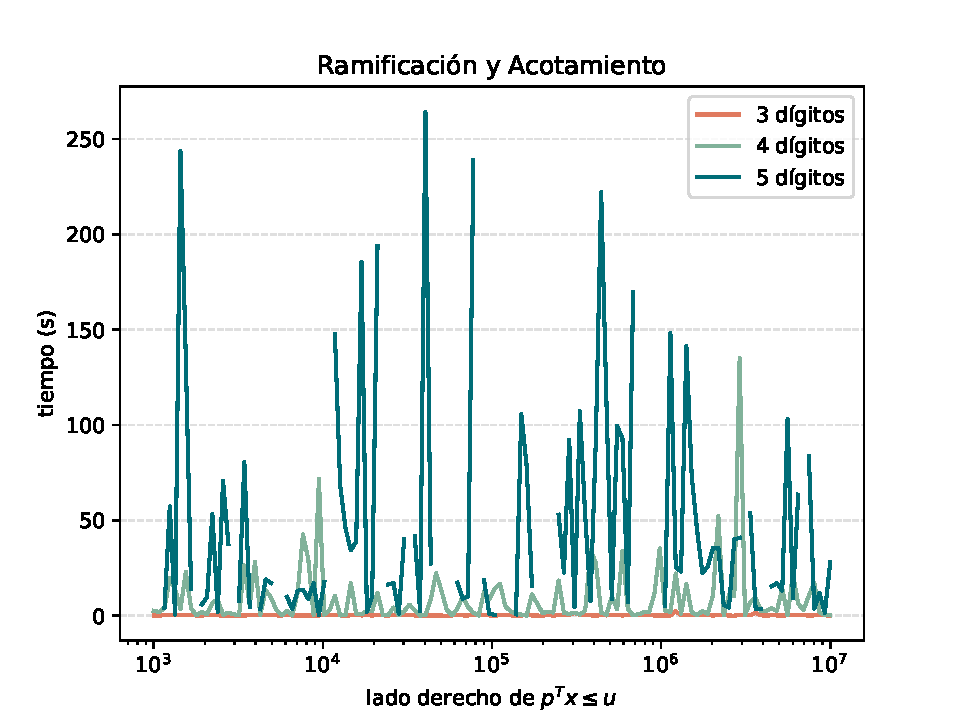
\includegraphics[width=\linewidth]{/home/tempdata/repos/thesis/static/inf/digits-bb_full.pdf}
  \end{subfigure}
  \hfill
  \begin{subfigure}{0.80\textwidth}
    \centering
    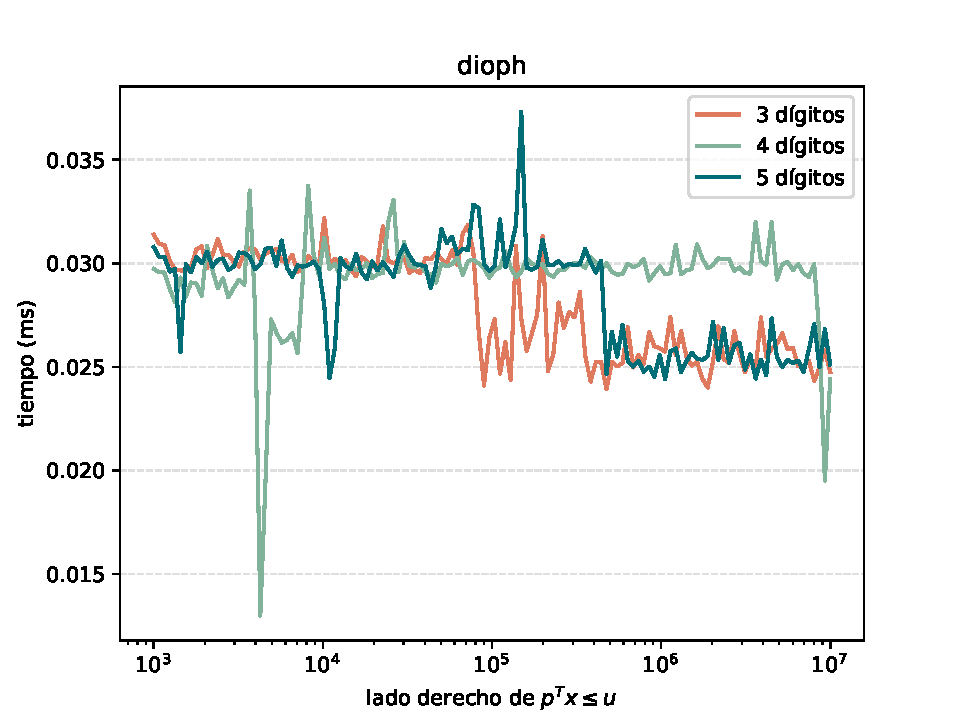
\includegraphics[width=\linewidth]{/home/tempdata/repos/thesis/static/inf/digits-dioph.pdf}
  \end{subfigure}

  \caption{Tiempos de terminación promedio cuando varía el presupuesto y el
			número de digitos. \textit{Arriba}: Resultados en segundos de R\&A. \textit{Abajo}:
			Resultados en milisegundos de nuestro método \texttt{dioph}.}
  \label{fig:exp:inf:rhs}
\end{figure}

Por los resultados obtenidos en las dos subsecciones anteriores, no sorprende que el algoritmo
\ref{algo:inf} tenga mejores tiempos de terminación que R\&A, y que no se vea afectado por la
precisión numérica del vector objetivo $\vec{p}$. Esto solo muestra que los tiempos de terminación
de R\&A son lentos para instancias de \eqref{theory:formulation}.

En realidad, nos interesa mostrar la inestabilidad numérica de R\&A a medida que la precisión del
vector objetivo $\vec{p}$ aumenta. Para ello, fijamos una de las $N = 128$ instancias y dividimos el
tiempo de terminación usando $\vec{p}_4$ entre el correspondiente tiempo usando $\vec{p}_3$; si
R\&A no encontró una solución en cualesquiera de los dos problemas, nos deshacemos de este
dato. Realizamos el mismo procedimiento entre $\vec{p}_5$ y $\vec{p}_4$.

Denominamos como multiplicadores a las razones anteriores, pues representan el factor de aumento en
los tiempos de terminación de R\&A cuando utilizamos una cifra decimal extra. La figura
\ref{fig:exp:inf:hist} muestra la distribución de estos multiplicadores. En el 60\% de los casos, el
multiplicador es al menos 10. Es decir, una cifra decimal extra en $\vec{p}$ provoca, en la mayoría
de los casos, que el tiempo de terminación en R\&A sea al menos diez veces mayor.

De acuerdo a la subsección anterior, deberíamos esperar que la gran mayoría de los multiplicadores
se concentren alrededor de $10^{n/2} = 100$. No obstante, solamente el 20\% de estos lo hace. El
autor hipotetiza que esto es causado por el uso de heurísticas en nuestra implementación de R\&A.
% TODO: contar cuántas instancias encontraron una solución gracias a las heurísticas.
% TODO: mostrar la distribución usando un solver sin heurísticas.

\begin{figure}[hbtp]
	\centering
    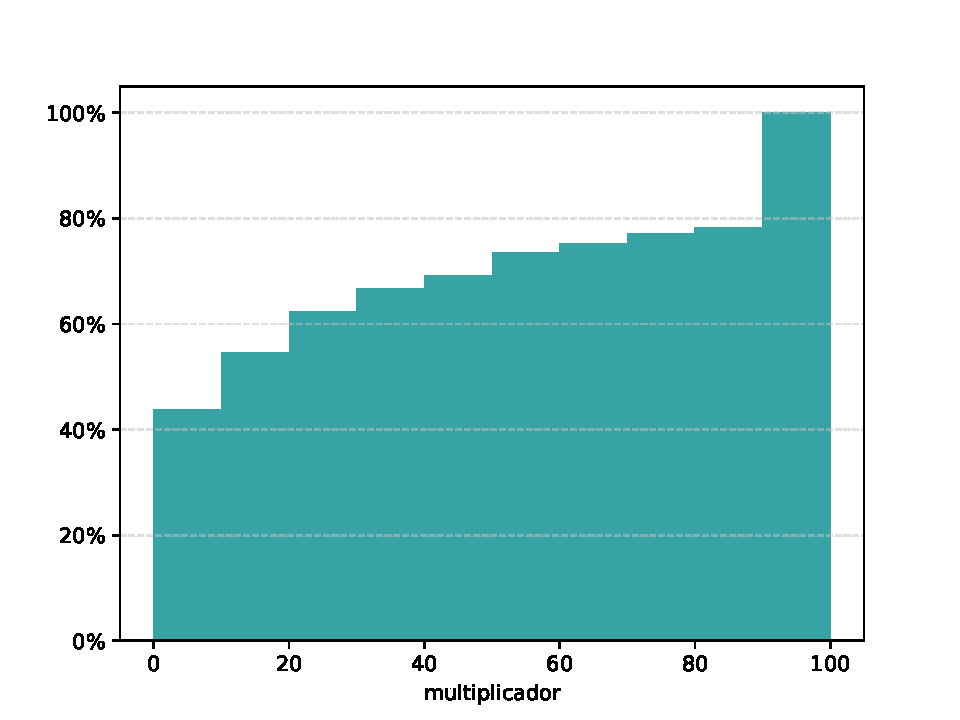
\includegraphics[width=\linewidth]{/home/tempdata/repos/thesis/static/inf/mult-hist-cum.pdf}
	\caption{Distribución de multiplicadores}
	\label{fig:exp:inf:hist}
\end{figure}
